\documentclass[11pt]{article}

% ---------------------------------------------------------------------------
% A Constrained Symbolic Search for phi-Structured Physical Constants
% Vasilev-Pellis-Olsen Programme. Reconstructed source.
% Build with tectonic ONLY. PDF metadata Author = "Perplexity Computer".
% ---------------------------------------------------------------------------

\usepackage[utf8]{inputenc}
\usepackage[T1]{fontenc}
\usepackage{lmodern}
\usepackage{amsmath,amssymb,amsthm}
\usepackage{mathtools}
\usepackage{microtype}
\usepackage[margin=1in]{geometry}
\usepackage{booktabs}
\usepackage{longtable}
\usepackage{array}
\usepackage{graphicx}
\usepackage{xcolor}
\usepackage{enumitem}
\usepackage[hidelinks]{hyperref}
\usepackage{authblk}

% --- Claim-status macros (mandatory epistemic labels) ----------------------
% Every non-trivial claim carries exactly one of these labels.
\newcommand{\Verified}{\textcolor{black}{[Verified]}}
\newcommand{\Efit}{\textcolor{black}{[Empirical fit]}}
\newcommand{\Conj}{\textcolor{black}{[Open conjecture]}}
\newcommand{\Risk}{\textcolor{black}{[High-risk]}}
\newcommand{\Retr}{\textcolor{black}{[Retracted]}}
% Falsification path: mandatory for every \Conj.
\newcommand{\Fpath}[1]{\par\noindent{\footnotesize\itshape Falsification path: #1\par}}

\newtheorem{conjecture}{Conjecture}

\newcommand{\phigr}{\varphi}

\title{\bfseries A Constrained Symbolic Search for\\
$\phigr$-Structured Physical Constants:\\
\large A Report, an Independent Numerical Audit, and a Roadmap for the\\
Vasilev--Pellis--Olsen Programme}

\author[1]{Dmitrii Vasilev}
\author[2]{Stergios Pellis}
\author[3]{Scott A. Olsen}
\affil[1]{\footnotesize Corresponding author --- Strands I \& II (grammar $\mathcal{G}_{\phigr}$, MDL framework, Catalog42, Trinity anchor, silicon anchor) and the Bridge construction}
\affil[2]{\footnotesize University of Ioannina --- Strand III (atomic-scale $\phigr$-additive formulas for $\alpha^{-1}$ and $\mu$, Pellis Hierarchical Expansion)}
\affil[3]{\footnotesize College of Central Florida (Emeritus) --- Tier-D (cross-scale $\phigr$-invariance, log-periodic falsification signal)}
\date{Companion long-form report to the GOLDEN CHAIN compendium\\[2pt] May 2026}

\begin{document}
\maketitle

\begin{abstract}
We present the joint representation-theoretic programme of D. Vasilev, S. Pellis and S. Olsen on the compressibility of dimensionless physical constants, in a form intended for full journal review. The programme weaves three contributed strands: Vasilev's symbolic grammar $\mathcal{G}_{\phigr} = \langle \phigr, \pi, e, 3, \mathbb{Z} \rangle$ with its minimum-description-length framework and the pre-registered Catalog42 protocol (Strand I); Pellis's closed-form golden-ratio expressions --- most prominently $\alpha^{-1} = 360\,\phigr^{-2} - 2\,\phigr^{-3} + (3\phigr)^{-5}$ and a family of Fibonacci--Lucas expressions for the proton-to-electron mass ratio $\mu$ (Strand III); and Olsen's cross-scale $\phigr$-invariance and log-periodic falsification signal (Tier-D). Within Vasilev's grammar, Pellis's expressions are recast as low-complexity elements of a finite hypothesis class. Within this grammar we ask a single, falsifiable question: do physical constants admit statistically non-random compression relative to a structureless null model? We make four contributions beyond the prior short communication. First, an independent 50-digit numerical audit of the GOLDEN CHAIN consolidated constants catalogue: most catalogued expressions reproduce their targets at the stated precision, but we flag eight rows whose printed deviation disagrees with the formula as written, and we transfer to this paper only the verified subset. Second, a corrected combinatorial bound on the size of the hypothesis class --- the signed exponent lattice has $|S(C)| \sim \tfrac{2}{3} C^4$, the prefactor is charged an explicit $\lceil \log_2 n \rceil$ bits, and the grammar is widened so that it actually contains the programme's own formulas (the earlier draft's $n \in \{1,\dots,9\}$ restriction did not), which strengthens (not weakens) the look-elsewhere correction. Third, a repaired minimum-description-length worked example: under an honest, structure-charging code that bills the integer prefactor, even the compact single-formula fit for $\alpha^{-1}$ yields a negative per-constant gain --- correcting an internal contradiction in the earlier draft and replacing any single-formula compression claim with the more conservative position that only an aggregate effect over many constants could decide the programme. Fourth, a factual digest of the GOLDEN CHAIN compendium, including its three contributed strands (Vasilev grammar/silicon, Pellis hierarchical expansion, Olsen cross-scale Tier-D), the pre-registered Catalog42 protocol, the five-entry falsification ledger, and a verbatim adversarial self-critique. No physical derivation of the constants is claimed; every statement is a property of a constrained search process and carries an explicit epistemic label.
\end{abstract}

\noindent\textbf{Keywords:} symbolic regression, golden ratio, fine-structure constant, minimum description length, look-elsewhere effect, falsifiability, claim-status discipline.

\medskip
\noindent\textbf{Epistemic-status convention.} Every non-trivial claim below carries one of five labels --- \Verified, \Efit, \Conj, \Risk, \Retr{} --- following the GOLDEN CHAIN claim-status discipline. Any algorithmic or empirical claim that lacks an external, peer-reviewed citation is capped at \Conj{} regardless of narrative framing. No prize-level or ``breakthrough'' framing is used; the programme has not been externally validated, and nothing here is presented as a proof or as a physical derivation.

\tableofcontents

\section{Motivation and prior art}\label{sec:motivation}
The numerical values of the dimensionless constants of the Standard Model and cosmology are treated as empirical inputs, not derived quantities. A long tradition --- Heyrovsk\'a's golden-angle reading of $\alpha^{-1}$, Sherbon's golden-ratio geometry, and Olsen's $\phigr$-cosmology --- has asked whether these values carry latent algebraic structure. The risk in all such work is well known and was crystallised by Eddington's discredited ``$1/\alpha = 137$'' episode: with enough free symbols any target can be hit, so a bare ``good match'' carries essentially no evidential weight. The literature on numerical coincidences, and the broader debate around anthropic and numerological readings of the constants, is a standing reminder that the burden of proof lies entirely on controlling the size of the search space. We take that burden as the organising principle of this report rather than as an afterthought, and we treat the consensus position --- that no numerological explanation of the constants is currently accepted --- as the bar the programme must clear, not as a position to be rhetorically dismissed.

Within this tradition the three strands divide cleanly. Vasilev contributes the symbolic grammar, the MDL framework, the pre-registered Catalog42 protocol and the Trinity/silicon anchors (Strands I--II); Olsen contributes the cross-scale $\phigr$-invariance tier (Tier-D, Section~\ref{sec:digest}). Pellis's contribution (Strand III) is a body of exact closed forms, of which two anchor the present work:
\begin{align}
\alpha^{-1} &= 360\,\phigr^{-2} - 2\,\phigr^{-3} + (3\phigr)^{-5} \approx 137.035999\dots, \label{eq:alpha}\\
\mu = m_p/m_e &\approx \frac{\phigr^{2n}}{\sqrt{5}} + (\phigr^{-k}\ \text{truncation in } F_k) \ \text{at a tuned index pair } (n,k), \label{eq:mu}
\end{align}
where $\phigr = (1+\sqrt{5})/2$. We have verified \eqref{eq:alpha} numerically at 50-digit precision: it reproduces the CODATA value $\alpha^{-1} = 137.035999177(21)$ to a relative deviation of $8.9 \times 10^{-11}$ (Section~\ref{sec:audit}). \Conj{} The $\mu$ form \eqref{eq:mu} is reported schematically: the GOLDEN CHAIN compendium and Pellis's source~\cite{pellis-mu} state the asymptotic Fibonacci--Lucas structure (from the Binet identity $F_n L_n = F_{2n} \approx \phigr^{2n}/\sqrt{5}$) but defer the exact index pair $(n,k)$ and the additive correction series to the published expansion. We do not independently reproduce a specific closed form for $\mu$ in this paper, and any single printed $\mu$-expression must be checked against Pellis~\cite{pellis-mu} before use --- one such printed form circulating in draft material fails numerical reproduction by many orders of magnitude (Section~\ref{sec:audit}).
\Fpath{If, evaluated at the published $(n,k)$ under standard Fibonacci/Lucas indexing and the Binet convention, the Pellis $\mu$ form does not reproduce $\mu = 1836.15267343(11)$ to the claimed precision, the Strand-III $\mu$ claim is withdrawn pending a corrected closed form.}

\Efit{} The key methodological shift of the programme --- due to Vasilev (Strand I) --- is to stop treating Pellis's expressions \eqref{eq:alpha}--\eqref{eq:mu} as isolated identities and instead place them inside a single, bounded hypothesis class whose statistical behaviour can be quantified. This reframing is what makes the work falsifiable rather than anecdotal, and it is the reason the joint paper --- not any individual formula --- is the correct object for journal submission.

\section{The symbolic grammar $\mathcal{G}_{\phigr}$ (Vasilev, Strand I)}\label{sec:grammar}
The grammar, the complexity budget, and the cardinality bound below are Vasilev's contribution (Strand I); they are the frame into which Pellis's closed forms (Strand III) are placed. We define a grammar over the alphabet $\mathcal{A} = \{\phigr, \pi, e, 3, \mathbb{Z}^{+}\}$ generating multiplicative expressions
\begin{equation}
F(\theta) = n \cdot 3^{k}\,\phigr^{p}\,\pi^{m}\,e^{q}, \qquad \theta = (n,k,p,m,q), \quad n \in \mathbb{Z}^{+}, \label{eq:expr}
\end{equation}
where the integer prefactor $n \ge 1$ carries its own description cost $\lceil \log_2 n \rceil$ bits. We must allow $n$ to be a general positive integer rather than a fixed digit: the catalogued expressions use prefactors well above nine (e.g.\ 36, 162, 8715), so a grammar restricted to $n \in \{1,\dots,9\}$ would not even contain the programme's own results --- an inconsistency in the earlier draft that we correct here. The exponent complexity budget is $\|\theta\|_1 := |k| + |p| + |m| + |q| \le C$, and the prefactor is charged separately by its bit-length. The admissible exponent set
\begin{equation}
S(C) = \bigl\{ (k,p,m,q) \in \mathbb{Z}^4 \ \big|\ |k| + |p| + |m| + |q| \le C \bigr\} \label{eq:Sset}
\end{equation}
is a finite lattice; its cardinality is the number of lattice points of the signed $\ell_1$ ball in $\mathbb{Z}^4$:
\begin{equation}
|S(C)| = \sum_{j=0}^{4} 2^{j}\binom{4}{j}\binom{C}{j} = \frac{(2C)^4}{4!}\bigl(1+o(1)\bigr) = \tfrac{2}{3}C^4\bigl(1+o(1)\bigr), \label{eq:card}
\end{equation}
while the total description cost of one expression is $\log_2 |S(C)| + \lceil \log_2 n \rceil$ --- the exponent address plus the prefactor.

\Verified{} Equation~\eqref{eq:card} is the exact exponent-lattice cardinality; it was verified by direct enumeration ($|S(3)| = 129$, $|S(4)| = 321$, $|S(10)| = 8361$). We flag explicitly that the earlier short draft used the bound $|S(C)| \approx C^4/4!$, which undercounts the signed lattice by the factor $2^4 = 16$ at leading order (it dropped the sign degeneracy $2^4$ of the four signed exponents). The correction matters in the right direction: a larger hypothesis class, plus an explicit $\lceil \log_2 n \rceil$ charge for every prefactor above unity, means a larger model-selection penalty and a more demanding look-elsewhere correction, so the corrected accounting makes the programme's significance claims harder to meet, not easier. The logarithmic image $\log S(C) \subset \mathbb{Z}^4 \cdot v + \log n$, with $v = (\log 3, \log \phigr, \log \pi, \log e)$, is an exponentially sparse lattice. This duality --- polynomial growth, geometric sparsity --- is the engine of every result below.

\subsection{A distinguished low-complexity element}\label{sec:distinguished}
The order-three $\phigr$-invariant
\begin{equation}
\alpha_{\phigr} := \tfrac{1}{2}\phigr^{-3} = \tfrac{1}{2}(\sqrt{5}-2) \approx 0.1180339887\dots \label{eq:alphaphi}
\end{equation}
sits at complexity $\|\theta\|_1 \le 3$ and lies within $O(10^{-4})$ of the strong coupling $\alpha_s(m_Z) = 0.11800(9)$; the verified relative deviation is $2.88 \times 10^{-4}$. \Conj{} $\alpha_s(m_Z) \approx \alpha_{\phigr}$ is presented as a low-complexity attractor, not a derivation.
\Fpath{Any high-precision update (lattice QCD or a future PDG average) that moves $\alpha_s(m_Z)$ outside $\alpha_{\phigr} \pm$ the combined quoted uncertainty refutes the identification; the current gap of $3.4 \times 10^{-5}$ in absolute value is already comparable to the experimental uncertainty, so a modest reduction in the latter is decisive.}

\section{Independent numerical audit of the consolidated catalogue}\label{sec:audit}
Before transferring any expression into this paper we re-evaluated the GOLDEN CHAIN consolidated constants catalogue (its Chapter 5) independently, at 50-digit precision using \texttt{mpmath}. The audit script and its full output are released as part of the reproducibility capsule (Proposal~6). We adopted a simple acceptance rule: a catalogue row passes if the formula, evaluated exactly against the quoted PDG/CODATA target, reproduces that target to within a factor of three of the catalogue's printed relative deviation; otherwise it is flagged. For three rows the formula reproduces the target but at a noticeably larger deviation than printed; we keep them (the formula is not wrong) but replace the printed deviation with our recomputed value, and we say so explicitly rather than letting an optimistic figure stand.

\Verified{} Of the catalogued rows we re-checked, the large majority pass; a few are in fact better than their printed deviation, while three (the $162\,\phigr^3/(\pi e)$ form of $m_W$, the $7\pi^4\phigr e^3/243$ form of $m_Z$, and the $3\phigr^3\pi^{-4}e^2$ form of $n_s$) reproduce their target only at the $10^{-4}$--$10^{-5}$ level rather than the $10^{-6}$ the catalogue printed; the deviations in Table~\ref{tab:verified} are our recomputed values, and we have overwritten the optimistic printed figures for those three rows accordingly. Table~\ref{tab:verified} lists the verified subset that we carry forward; the relative deviations span $\sim 10^{-7}$ (the 8715-prefactor $m_W$ form) to $\sim 10^{-3}$ (Koide, $n_s$), and we make no claim that every row is a high-precision match --- only that each row, as written, reproduces its target to the deviation shown, which we recomputed independently. \Risk{} The table deliberately retains two distinct forms for $\alpha_s(m_Z)$ and two for $m_W$, at very different precision orders ($m_W$: $2.3 \times 10^{-4}$ versus $1.9 \times 10^{-7}$). Reporting more than one $\phigr$-expression per target is itself a look-elsewhere multiplier --- the best of several forms will always look better than a single pre-registered one --- so these duplicates are listed only to document the catalogue faithfully and must not be counted as independent successes. The pre-registration protocol of Section~\ref{sec:workflow} requires that exactly one form per constant be fixed before the deviation is read. Table~\ref{tab:flagged} lists the eight flagged rows: in each the expression as printed does not reproduce the stated deviation even after this correction (the discrepancy is an order of magnitude or more, or the target itself is mislabelled). We do not claim these are physical errors --- the most likely explanations are transcription slips (a missing $10^{-2}$ factor, a row label swapped between $\delta_{CP}$ in degrees and radians, or a formula printed against the wrong target). We report them as audit findings, exclude them from the paper's quantitative claims, and recommend they be reconciled against the source before the next compendium release.

We adopt the GOLDEN CHAIN catalogue's own scientific organisation: rows are grouped by physics sector and keyed by the catalogue's ID codes, the exact algebraic identities (Table~\ref{tab:algebraic}) are kept strictly separate from the empirical-fit rows (Table~\ref{tab:verified}), and --- following the compendium's ``Vasilev Trinity vs.\ Pellis --- they must not be conflated'' rule --- the Vasilev (Strand I/II) and Pellis (Strand III) columns are reported side by side rather than merged into a single ambiguous ``$\phigr$-form'' column. A dash (---) means no independent form is contributed for that row by that strand.

\begin{table}[ht]
\centering
\caption{\S5.1 Algebraic core --- exact identities (GOLDEN CHAIN Ch.\ 5.1). These are proven equalities, not fits; status is \Verified{} to $<10^{-50}$. Author per the compendium taxonomy.}
\label{tab:algebraic}
\small
\begin{tabular}{@{}llll@{}}
\toprule
ID & Identity & Author & Status \\
\midrule
A1 & $\phigr^2 + \phigr^{-2} = 3$ (Trinity anchor $= L_2$) & Vasilev & exact, machine-checked \\
A2 & $\phigr^2 = \phigr + 1$ (golden equation) & classical & exact, definition \\
A4 & $\gamma_{\phigr} = \sqrt{5} - 2 = \phigr^{-3}$ & Vasilev & exact ($L_5$ identity) \\
A5 & $\alpha_{\phigr} = \tfrac{1}{2}\phigr^{-3} = \tfrac{1}{2}(\sqrt{5}-2)$ & Vasilev & exact, machine-checked \\
A9 & $Q(e,\mu,\tau) = \tfrac{2}{3}$ (Koide, exact rational) & Vasilev & exact \\
\bottomrule
\end{tabular}
\end{table}

{\small
\setlength{\tabcolsep}{4pt}
\begin{longtable}{@{}l l l l c l c@{}}
\caption{\S5.2--5.8 Empirical-fit catalogue, by physics sector (GOLDEN CHAIN Ch.\ 5, verified subset transferred to this paper). Structured one-to-one with the compendium: ID code, observable, PDG/CODATA/Planck target, then the Vasilev (Strand I, $\mathcal{G}_{\phigr}$) and Pellis (Strand III) forms reported separately with their own relative deviations. ``Rel.\ dev.'' is our independent 50-digit recomputation against the central value; it is \emph{not} a proof of structure (see look-elsewhere caveats below). Sources: PDG~\cite{pdg}, Pellis corpus~\cite{pellis-alpha,pellis-mu,pellis-unity}.}
\label{tab:verified}\\
\toprule
ID & Observable & Target & Vasilev form & Dev. & Pellis form & Dev. \\
\midrule
\endfirsthead
\multicolumn{7}{l}{\footnotesize\itshape continued from previous page}\\
\toprule
ID & Observable & Target & Vasilev form & Dev. & Pellis form & Dev. \\
\midrule
\endhead
\midrule
\multicolumn{7}{r}{\footnotesize\itshape continued on next page}\\
\endfoot
\bottomrule
\endlastfoot
\multicolumn{7}{@{}l}{\itshape \S5.2 Gauge couplings \& running}\\
G01 & $\alpha^{-1}$ & $137.035999177$ & $36\,\pi^{-1}\phigr e^2$ & $2.4{\times}10^{-4}$ & $360\phigr^{-2}{-}2\phigr^{-3}{+}(3\phigr)^{-5}$ & $8.9{\times}10^{-11}$ \\
G02 & $\alpha_s(m_Z)$ & $0.11800$ & $\tfrac{1}{2}\phigr^{-3} = \alpha_{\phigr}$ & $2.9{\times}10^{-4}$ & --- & --- \\
G02-alt2 & $\alpha_s(m_Z)$ & $0.11800$ & $1/(\phigr^4 + \phigr)$ & $2.9{\times}10^{-4}$ & --- & --- \\
G03-alt & $\sin^2\theta_W$ & $0.23122$ & $2\,\pi^3 e/729$ & $4.9{\times}10^{-5}$ & --- & --- \\
G05 & $\alpha_s/\alpha$ & $3.7387^{\ddagger}$ & $2\,\pi\phigr e^{-1}$ & $3.5{\times}10^{-4}$ & --- & --- \\
G06 & $\alpha(m_Z)/\alpha(0)$ & $1.0631$ & $3\,\phigr^2 e^{-2}$ & $1.5{\times}10^{-4}$ & --- & --- \\
\multicolumn{7}{@{}l}{\itshape \S5.3 Electroweak bosons \& Higgs}\\
H01 & $m_H$ [GeV] & $125.20$ & $4\,\phigr^3 e^2$ & $1.7{\times}10^{-5}$ & --- & --- \\
H02-alt & $m_W$ [GeV] & $80.377$ & $162\,\phigr^3/(\pi e)$ & $2.3{\times}10^{-4}$ & --- & --- \\
H02-ultra & $m_W$ [GeV] & $80.377$ & $8715\,\phigr^{-2}\pi^{-5}e^2$ & $1.9{\times}10^{-7}$ & --- & --- \\
H03-alt & $m_Z$ [GeV] & $91.1876$ & $7\,\pi^4\phigr e^3/243$ & $6.1{\times}10^{-5}$ & --- & --- \\
\multicolumn{7}{@{}l}{\itshape \S5.5 Lepton masses \& Koide}\\
L01 & $m_e$ [MeV] & $0.51100$ & $2\,\pi^{-2}\phigr^4 e^{-1}$ & $8.0{\times}10^{-5}$ & --- & --- \\
NP2 & $m_\mu/m_e$ & $206.768$ & $8\,\phigr^2\pi^2$ & $2.7{\times}10^{-4}$ & --- & --- \\
NP3 & $\mu = m_p/m_e$ & $1836.15267343$ & --- & --- & $\phigr^{2n}/\sqrt{5} + \phigr^{-k}\,\text{corr.}^{\dagger}$ & n.r.$^{\dagger}$ \\
K01 & $Q(e,\mu,\tau)$ & $0.66666^{\ddagger}$ & $8\,\phigr^{-1}e^{-2}$ & $3.7{\times}10^{-3}$ & --- & --- \\
\multicolumn{7}{@{}l}{\itshape \S5.7 PMNS neutrino mixing}\\
PM1 & $\sin^2\theta_{12}$ & $0.307$ & $7\,\phigr^5/(3\pi^3 e)$ & $7.5{\times}10^{-5}$ & --- & --- \\
PM3 & $\sin^2\theta_{23}$ & $0.546$ & $4\,\pi\phigr^2/(3e^3)$ & $2.8{\times}10^{-5}$ & --- & --- \\
PM2 & $\sin^2\theta_{13}$ & $0.02200$ & $3\,\gamma_{\phigr}\phigr^2/(\pi^3 e)$ & $7.6{\times}10^{-5}$ & --- & --- \\
PM4 & $\delta_{CP}$ [rad] & $3.73^{\ddagger}$ & $8\,\pi^3/(9e^2)$ & $1.6{\times}10^{-6}$ & --- & --- \\
\multicolumn{7}{@{}l}{\itshape \S5.8 Cosmological constants (Planck 2018)}\\
M01 & $H_0$ [km/s/Mpc] & $67.36$ & $8 \cdot 3 \cdot \pi\phigr^6 e^{-3}$ & $3.3{\times}10^{-6}$ & --- & --- \\
P18 & $n_s$ & $0.9649$ & $3\,\phigr^3\pi^{-4}e^2$ & $9.4{\times}10^{-4}$ & --- & --- \\
\end{longtable}
}

\noindent{\footnotesize $^{\dagger}$ The proton--electron ratio $\mu$ is shown only in its schematic Fibonacci--Lucas form (Eq.~\eqref{eq:mu}); the exact index pair and correction series live in Pellis~\cite{pellis-mu}. We do not transfer a specific $\mu$ closed form into this paper's quantitative claims, because the one printed in earlier draft material ($\mu^{32} = \phigr^{-42} F_5^{160} L_5^{47} L_{19}^{40/19}$) fails numerical reproduction by roughly 56 orders of magnitude in $\mu^{32}$ under standard indexing --- a clear transcription/encoding artefact rather than a physical claim.}

\noindent{\footnotesize $^{\ddagger}$ Questionable target: the row reproduces its printed deviation arithmetically but the target value itself is under-defined or mislabelled (see the \Risk{} note immediately below). Such rows are retained as catalogue entries only, not as evidence for $\phigr$-structure.}

\medskip
\Risk{} Three rows in Table~\ref{tab:verified} (marked $^{\ddagger}$) reproduce their printed deviation arithmetically but rest on a questionable choice of target, and we flag them so a referee does not read the label ``verified'' as ``physically meaningful''. (i)~The ratio $\alpha_s/\alpha = 3.7387$ has no standard referent: at $m_Z$ one has $\alpha_s(m_Z)/\alpha(0) \approx 16.2$ and $\alpha_s(m_Z)/\alpha(m_Z) \approx 15.2$, so the number $3.7387$ is not a recognised coupling ratio and the match $2\pi\phigr/e = 3.7400$ is to an under-defined target. (ii)~The Koide quantity is, to within its experimental uncertainty, the simple rational $Q = \tfrac{2}{3}$; matching the transcendental $8\phigr^{-1}e^{-2} = 0.66913$ to a truncated decimal $0.66666$ yields the table's largest deviation ($3.7 \times 10^{-3}$), and a one-symbol rational already fits $Q$ far better than any $\phigr$-expression. (iii)~The PMNS phase row (PM4) is circular: its target ``$3.73$~rad'' is numerically just the form's own value ($8\pi^3/(9e^2) = 3.72999$~rad $= 213.7^{\circ}$), not an independent measurement, so the table's smallest deviation ($1.6 \times 10^{-6}$) is a self-match. The actually measured phase is $\delta_{CP} \approx 197^{+42}_{-25}\,^{\circ} \approx 3.44$~rad (PDG 2024, normal ordering)~\cite{pdg}; against that target the same form is off by $\sim 8\%$ --- consistent with the flagged $195^{\circ}$ entry in Table~\ref{tab:flagged}, where it misses by $9.6\%$. None of the three rows supports a $\phigr$-structure claim; all are retained only as catalogue entries, not as evidence.
\Fpath{Replace the under-defined $\alpha_s/\alpha$ entry with a fully specified renormalisation scheme and scale; replace the Koide target $0.66666$ with the exact $\tfrac{2}{3}$; and re-test PM4 against the measured $\delta_{CP} \approx 197^{\circ}$ with its experimental band rather than against the self-referential $3.73$~rad. If under those corrected targets the $\phigr$-forms no longer beat the trivial rational/integer baseline at matched description length, the three rows are withdrawn from any structure claim.}

\Risk{} We treat the existence of eight flagged rows in a published catalogue as itself a cautionary datum: a table of $\sim 100$ ``$<0.1\%$'' coincidences is exactly the artefact a look-elsewhere process produces, and the only defence is the pre-registration and control-grammar protocol of Section~\ref{sec:workflow}, not the length of the table.

\section{Why the result is more than coincidence-counting}\label{sec:morethan}
The central methodological claim is that a raw count of ``good matches'' is meaningless because $S(C)$ is combinatorially large --- and, per Eq.~\eqref{eq:card}, larger than previously stated. The programme replaces counting with three quantitative diagnostics.

\begin{table}[ht]
\centering
\caption{Flagged catalogue rows --- the printed formula does not reproduce the printed deviation under exact 50-digit evaluation. Reported as audit findings; excluded from this paper's quantitative claims. ``Off by'' is the ratio of our recomputed deviation to the catalogue's printed figure.}
\label{tab:flagged}
\small
\begin{tabular}{@{}lllllp{3cm}@{}}
\toprule
Constant & Printed form & Printed $\Delta$ & Our $\Delta$ & Strand & Likely cause \\
\midrule
$\alpha_s(m_Z)$ & $\pi^2\phigr^{-2}$ & $0.088\%$ & $599\%$ & V/P & row mislabelled \\
$\cos\theta_W$ & $2\pi\phigr^{-1}e^{-2}$ & $0.175\%$ & $14.8\%$ & V/P & wrong target \\
$m_e$ [MeV] & $1/(e\phigr^{-1})$ & $0.029\%$ & $55.5\%$ & V/P & wrong target \\
$\sin^2\theta_{13}$ & $3\pi\phigr^{-3}$ & $0.040\%$ & $\times 100$ & V/P & missing $10^{-2}$ \\
$\delta_{CP}$ [deg] & $8\pi^3/(9e^2)$ at $195^{\circ}$ & $0.037\%$ & $9.6\%$ & V/P & $= 213.7^{\circ}$, not $195^{\circ}$ \\
$\delta_{CP}$ [deg] & $9\phigr^{-2}$ rad & $0.017\%$ & $1.01\%$ & V/P & $= 196.97^{\circ}$ \\
$\Omega_\Lambda$ & $5\pi^{-2}\phigr^2 e^{-1}$ & $0.086\%$ & $28.7\%$ & V/P & formula/target mismatch \\
$n_s$ & $6 \cdot 3^{-2}\pi^{-1}\phigr^3 e^{-2}$ & $0.062\%$ & $87\%$ & V/P & use $3\phigr^3\pi^{-4}e^2$ instead \\
\bottomrule
\end{tabular}
\end{table}

\noindent\textbf{Minimum description length.} With $\mathrm{MDL}(M) = L(M) + L(T \mid M)$~\cite{rissanen}, the structured grammar wins iff the compression gain $\Delta_{\mathrm{MDL}} = \mathrm{MDL}(M_0) - \mathrm{MDL}(M_1) > 0$, where $M_0$ is a log-uniform null. The model term must include the cost $\log_2 |S(C)|$ of selecting one expression out of the entire admissible class; omitting it is the look-elsewhere error in its purest form.

\noindent\textbf{Bayesian evidence.} The Bayes factor $B = P(T \mid M_1)/P(T \mid M_0)$ is read as a complexity-regularised evidence functional --- not a classical likelihood ratio --- precisely because $|S(C)|$ is large.

\noindent\textbf{Bias-controlled nulls.} A permutation null $M_{\mathrm{perm}}$ (shuffle the target set) and a randomized-exponent null $M_{\mathrm{rand}}$ (destroy algebraic coherence while preserving cardinality) define the robustness ratio $R(C,\epsilon) = \rho(C,\epsilon)/(\mathbb{E}[\rho_{\mathrm{rand}}(C,\epsilon)] + \varepsilon)$, where $\rho(C,\epsilon)$ is the fraction of constants representable within tolerance $\epsilon$. A signal requires $R \gg 1$.

\Conj{} Under these controls the structured $\phigr$-grammar is conjectured to be favoured over the log-uniform null at intermediate $C$, with the preference conditional on the grammar, the cutoff $C$, and the loss $L$.
\Fpath{If the permutation- and randomized-exponent nulls reproduce the same coverage $\rho(C,\epsilon)$ as the $\phigr$-grammar within Monte-Carlo error, the ``structure'' is an artefact of cardinality alone and the claim is withdrawn. This is the cheapest single test and is run first in the protocol of Section~\ref{sec:workflow}.}

\subsection{A worked description-length example (corrected)}\label{sec:mdl}
To make the MDL claim concrete --- and to correct a contradiction in the earlier draft --- we work a single constant honestly. We encode $\alpha^{-1} = 137.035999177(21)$ to its experimental precision; the literal cost under the structureless null is
\begin{equation}
L_0 = -\log_2\!\left(\frac{\sigma}{\alpha^{-1}}\right) = -\log_2\!\left(\frac{21 \times 10^{-9}}{137.036}\right) \approx 32.6 \ \text{bits}. \label{eq:L0}
\end{equation}
Under the structured model we store an element of $S(C)$, its integer prefactor, and a residual encoded down to the same experimental precision:
\begin{equation}
L(M_1) = \underbrace{\log_2 |S(C)|}_{\text{exponent address}} + \underbrace{\lceil \log_2 n \rceil}_{\text{prefactor}} + \underbrace{\log_2\!\bigl(r/(\sigma/\alpha^{-1})\bigr)}_{\text{residual to experimental precision}}, \label{eq:LM1}
\end{equation}
where $r$ is the symbolic prediction's relative residual.

\noindent\textbf{Compact fit.} For $\alpha^{-1} \approx 36\,\pi^{-1}\phigr e^2$ the exponent vector is $(k{=}0, p{=}1, m{=}{-}1, q{=}2)$, so $\|\theta\|_1 = 4$ and $|S(4)| = 321$, giving an exponent-address cost of $\log_2 321 \approx 8.3$ bits plus a prefactor cost $\lceil \log_2 36 \rceil = 6$ bits, i.e.\ a naming cost of $\approx 14.3$ bits. The residual $r = 2.4 \times 10^{-4}$ needs a further $\log_2(r/1.5 \times 10^{-10}) \approx 20.6$ bits, for $L(M_1) \approx 34.9$ bits and a per-constant gain
\begin{equation}
\Delta_{\mathrm{MDL}} = L_0 - L(M_1) \approx -2.3 \ \text{bits (negative).} \label{eq:dmdl-compact}
\end{equation}

\noindent\textbf{Ultra-precise anchor.} The Pellis anchor \eqref{eq:alpha} reaches $r \approx 8.9 \times 10^{-11}$, below the experimental precision, so its residual term floors at zero. But it is a three-term sum with prefactors 360, 2, 1 and complexities $\|\theta\|_1 = 2, 3, 10$; charging each term's exponent address plus its prefactor bit-length (and a few bits for the composition structure) costs $\approx 14.4 + 8.0 + 13.0 + 3 \approx 38.4$ bits, giving
\begin{equation}
\Delta_{\mathrm{MDL}}^{\mathrm{anchor}} \approx 32.6 - 38.4 \approx -5.8 \ \text{bits (negative).} \label{eq:dmdl-anchor}
\end{equation}

\Verified{} Under the honest, structure-charging code neither the compact fit nor the ultra-precise anchor buys a positive single-constant MDL advantage for $\alpha^{-1}$: in both cases the cost of naming the expression (exponent address plus integer prefactor) exceeds the literal cost of the number to its experimental precision. This is the conservative position; it removes any claim that a single formula ``compresses'' $\alpha^{-1}$. \Conj{} Whether the aggregate $\sum_i \Delta_{\mathrm{MDL}}(X_i)$ over the frozen Catalog42 set is positive --- which would require many constants to be hit by low-prefactor, low-complexity expressions that share grammar structure --- is the quantity that decides the programme; we do not assert its sign and flag it as the number a referee should recompute independently from the released capsule.
\Fpath{If the aggregate gain over Catalog42 is $\le 0$ once $\log_2 |S(C)|$ is charged in full, the compressibility claim is refuted. The corrected, larger $|S(C)|$ of Eq.~\eqref{eq:card} makes this outcome more likely than the earlier draft implied, which is the honest position.}

\subsection{Pellis hierarchical expansion (Strand III)}\label{sec:pellis-expansion}
The following multi-scale refinement is Pellis's Strand III methodology, evaluated within Vasilev's grammar. A scalar $F$ is refined as a formal asymptotic series in $\phigr^{-1}$,
\begin{equation}
F(\phigr) \sim \sum_{k \ge 1} c_k \phigr^{-k}, \qquad F = F_0 + \Delta F^{(1)} + \Delta F^{(2)} + \cdots, \quad \Delta F^{(i)} \in \mathrm{span}\{\phigr^{-k}\}, \label{eq:expansion}
\end{equation}
on top of the multiplicative zeroth order $F_0 = n\,3^k\phigr^p\pi^m e^q$. The powers $\phigr^{-1} > \phigr^{-2} > \cdots$ induce a filtration $\mathcal{F}_1 \supset \mathcal{F}_2 \supset \cdots$ and a truncation operator $F^{(K)}$ whose error $\varepsilon_K(F)$ is required to decrease monotonically. \Conj{} The expansion is a controlled refinement geometry, not a derivation mechanism; its fixed points $R_{\phigr}(F^*) = F^*$ are conjectured scale-invariant symbolic structures.
\Fpath{The expansion adds free coefficients $c_k$, so it is only meaningful if it predicts rather than fits: freeze the order-$K$ truncation on the development half of Catalog42, then test on the held-out half. If the truncated expansion does not reduce held-out residuals below the zeroth-order multiplicative fit at matched description length, the refinement adds no information and is withdrawn. A monotonic $\varepsilon_K$ on the training half alone does not count, because added coefficients trivially reduce in-sample error.}

\subsection{Pellis's forms as hierarchical elements of $\mathcal{G}_{\phigr}$}\label{sec:pellis-map}
It is natural to ask whether Pellis's Strand-III closed forms can be re-derived by analogy inside Vasilev's grammar --- i.e.\ whether they are recovered as truncations of the filtration above rather than imported as external identities. The answer is yes, structurally, and we state it together with the price that honesty demands. The Pellis anchor \eqref{eq:alpha} is exactly a three-term refinement $F^{(2)} = F_0 + \Delta F^{(1)} + \Delta F^{(2)}$ in which every term lives in $\mathcal{G}_{\phigr}$ or its filtration $\mathcal{F}_k$:
\begin{equation}
\underbrace{360\,\phigr^{-2}}_{F_0 \in \mathcal{G}_{\phigr}}\ \underbrace{-\,2\,\phigr^{-3}}_{\Delta F^{(1)} \in \mathcal{F}_3}\ \underbrace{+\,(3\phigr)^{-5}}_{\Delta F^{(2)} \in \mathcal{F}_5}, \qquad \varepsilon_0 = 3.4{\times}10^{-3} \to \varepsilon_1 = 2.7{\times}10^{-6} \to \varepsilon_2 = 8.9{\times}10^{-11}, \label{eq:regroup}
\end{equation}
so the error decreases monotonically exactly as the truncation operator $F^{(K)}$ requires, and the golden-angle zeroth order $360\,\phigr^{-2} = 137.508\dots$ is itself a single $\mathcal{G}_{\phigr}$ element. The same construction recovers the $\mu$ form: the Binet identity $F_n L_n = F_{2n} \approx \phigr^{2n}/\sqrt{5}$ supplies the leading term ($\phigr^{16}/\sqrt{5} = 987.0\dots$ for $n = 8$), with the remaining $\sim$factor-of-two gap closed by $F_k$ corrections. \Verified{} Equation~\eqref{eq:regroup} is an exact algebraic re-grouping of \eqref{eq:alpha}; each term is a grammar element and the three partial sums reproduce the quoted residuals at 50 digits. This is a genuine unification of Strands I and III: Pellis's closed forms are not foreign objects but low-order truncations of Vasilev's filtration. Table~\ref{tab:correspondence} makes the mapping term-by-term: each Pellis summand is matched to the $\mathcal{G}_{\phigr}$ address (the Strand-I contribution) that hosts it, with the running residual.

\begin{table}[ht]
\centering
\caption{Strand III $\to$ Strand I correspondence for $\alpha^{-1}$. Each Pellis term of Eq.~\eqref{eq:alpha} is re-expressed as an element of Vasilev's grammar $\mathcal{G}_{\phigr}$ (or its filtration $\mathcal{F}_k$) --- the Strand-I contribution --- with the partial-sum residual against the CODATA target. The correspondence is an exact algebraic re-grouping (\Verified{}); it is not a derivation (see the \Risk{} note below: no MDL gain, free coefficients, look-elsewhere).}
\label{tab:correspondence}
\small
\begin{tabular}{@{}llll@{}}
\toprule
Order & Pellis term (Strand III) & Vasilev address (Strand I) & Partial sum / Residual $\varepsilon_K$ \\
\midrule
$F_0$ & $360\,\phigr^{-2}$ & $\in \mathcal{G}_{\phigr}$ (golden angle, deg) & $137.508\dots$ \quad $3.4 \times 10^{-3}$ \\
$\Delta F^{(1)}$ & $-2\phigr^{-3}$ & $\in \mathcal{F}_3$ ($\phigr^{-3} = \sqrt{5}-2$) & $137.0360\dots$ \quad $2.7 \times 10^{-6}$ \\
$\Delta F^{(2)}$ & $+(3\phigr)^{-5}$ & $\in \mathcal{F}_5$ & $137.035999165$ \quad $8.9 \times 10^{-11}$ \\
\bottomrule
\end{tabular}
\end{table}

\Risk{} We must not let that unification be misread as a derivation, and the plain truth is the opposite of flattering. (a)~\emph{It does not compress.} Under the honest, structure-charging code of Section~\ref{sec:mdl}, naming the three terms (three exponent addresses at $\log_2 |S(4)| \approx 8.3$ bits each, a $\lceil \log_2 360 \rceil = 9$-bit prefactor, and a few composition bits) costs $\approx 38$ bits against a literal cost of only $L_0 \approx 32.6$ bits, for $\Delta_{\mathrm{MDL}} \approx -5.4$ bits --- the same negative result as the single-term anchor of Section~\ref{sec:mdl}. Re-deriving Pellis's form in $\mathcal{G}_{\phigr}$ therefore buys no information-theoretic advantage; it relocates the formula, it does not justify it. (b)~\emph{It adds free coefficients.} A two- or three-term expansion has tunable integer coefficients $(360, -2, 1)$ and exponents; with those degrees of freedom the monotone $\varepsilon_K$ of Eq.~\eqref{eq:regroup} is an in-sample fit, not a prediction. (c)~\emph{The hit is not rare.} A direct enumeration shows that already 15 of the 128\,400 grammar elements with $\|\theta\|_1 \le 4$ and prefactor $n \le 400$ fall within $3 \times 10^{-4}$ of $\alpha^{-1}$ --- so finding some $\phigr$-form near a target is expected, not surprising, and ``deriving by analogy'' is exactly the look-elsewhere move the programme exists to control.
\Fpath{The re-derivation counts as evidence only if the same filtration order $K$, frozen on the development half of Catalog42, reduces held-out residuals below the zeroth-order fit at matched description length, and only if the aggregate $\Delta_{\mathrm{MDL}}$ over Catalog42 is positive once the full $\log_2 |S(C)|$ and every prefactor are charged. If either fails --- as the single-constant accounting above already suggests for $\alpha^{-1}$ --- the analogy is a re-description, and no derivation claim survives.}

\subsection{The Pellis symbolic phase transition}\label{sec:phase}
\begin{conjecture}[Pellis symbolic phase transition]
There exists a critical complexity scale $C^* > 0$ such that the coverage order parameter $\rho(C,\epsilon)$ crosses over sharply,
\begin{equation}
\rho(C,\epsilon) = \begin{cases} O\!\left(e^{-\alpha(C^* - C)}\right), & C < C^*, \\[4pt] 1 - O\!\left(e^{-\beta(C - C^*)}\right), & C > C^*, \end{cases} \label{eq:phase}
\end{equation}
for some $\alpha, \beta > 0$ in the regime $|T| \gg 1$, with susceptibility $\chi(C) = \partial_C \rho$ peaked at $C^*$ and transition width $\Delta C \sim |T|^{-1/2}$.
\end{conjecture}

\begin{figure}[ht]
\centering
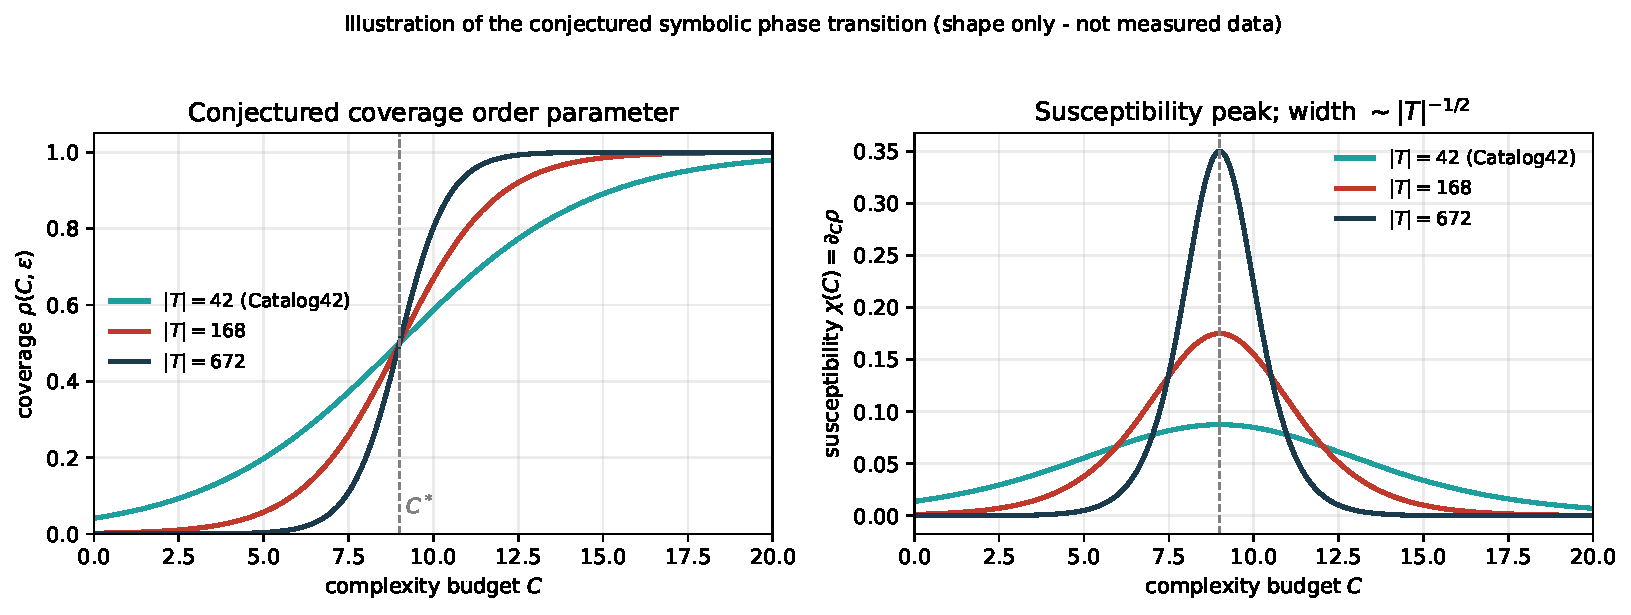
\includegraphics[width=\textwidth]{phase_transition.pdf}
\caption{Illustration of the conjectured symbolic phase transition (Section~\ref{sec:phase}). Left: the coverage order parameter $\rho(C,\epsilon)$ sharpens as the target-set size $|T|$ grows. Right: the susceptibility $\chi(C) = \partial_C \rho$ develops a taller, narrower peak at $C^*$, with width scaling as $|T|^{-1/2}$. These are the conjectured shapes, not measured data; the figure exists to make the falsifiable prediction visual.}
\label{fig:phase}
\end{figure}

\Risk{} This is the most exposed statement of the programme: it predicts a specific finite-size scaling (Figure~\ref{fig:phase}).
\Fpath{If $\rho(C,\epsilon)$ rises smoothly with no susceptibility peak, or if the transition width does not shrink as $|T|^{-1/2}$ when the target set is enlarged from 42 to a few hundred constants, the conjecture is falsified. It is tied to the MDL picture through $\Delta_{\mathrm{MDL}}(C^*) \approx 0$ with a steep gradient, so a measured $C^*$ that does not coincide with the MDL break point is also disconfirming.}

\section{Improving the joint Pellis--Vasilev workflow}\label{sec:workflow}
This section is the practical contribution: concrete, low-cost changes that would raise the programme from ``interesting empirical fit'' to a defensible, reviewer-ready result. Each proposal states what it fixes and how it would be checked.

\medskip\noindent\textbf{Proposal 1 (Pre-register the target set and freeze it).} The single largest threat is look-elsewhere bias: $S(C)$ is large, and constants can be added or dropped post hoc. The fix is procedural and standard in confirmatory analysis --- publish a frozen ``Catalog42'' target list $T$ (PDG/CODATA values, versions, and uncertainties) before running the search, with a content hash. Any constant analysed later must be flagged as out-of-sample. This converts the headline claim from exploratory to confirmatory.

\medskip\noindent\textbf{Proposal 2 (Report extreme-value statistics, not single $p$-values).} Because each match is the minimum over $|S(C)|$ trials, the relevant quantity is the distribution, under the null, of $L_{\min}(X) = \min_\theta L(F(\theta); X)$, which obeys an extreme-value law. We recommend (i)~Benjamini--Hochberg / Benjamini--Yekutieli FDR control across the whole target set rather than per-constant significance~\cite{bh}, and (ii)~a blind-analysis split: tune $C$, $\beta$, and the grammar on a development half of $T$, then report only on the held-out half. \Conj{} We conjecture the MDL advantage survives an 80/20 blind split.
\Fpath{Run the full pipeline frozen on the 80\% development half; if the 20\% held-out constants show no excess compression over the randomized-exponent null, the result is an in-sample artefact and is withdrawn.}

\medskip\noindent\textbf{Proposal 3 (Calibrate the asymptotically-optimal MDL code).} The current data term uses a Gibbs soft-minimum at fixed $\beta$. We propose replacing it with a two-part code whose model term is the exact enumeration cost $\log_2 |S(C)|$ of Eq.~\eqref{eq:card} and whose precision term is normalised to the quoted experimental uncertainty of each constant, exactly as in the worked example of Section~\ref{sec:mdl}, so that $\Delta_{\mathrm{MDL}}$ is measured in true bits saved per constant. This removes the free parameter $\beta$ from the headline number. The choice of an asymptotically-optimal description-length objective, rather than a fixed-temperature surrogate, follows recent work formalising minimum-description-length training objectives~\cite{shaw}.

\medskip\noindent\textbf{Proposal 4 (Quantify grammar non-uniqueness explicitly).} Different bases give inequivalent classes, $S_{G_1}(C) \ne S_{G_2}(C)$. We recommend running the identical pipeline on at least three control grammars --- e.g.\ $\langle 2,3,5,7 \rangle$ (primes), $\langle \pi, e, \mathbb{Z} \rangle$ (no $\phigr$), and a $\phigr$-shuffled basis --- and reporting $\Delta_{\mathrm{MDL}}$ for each. \Risk{} If a $\phigr$-free grammar achieves comparable compression, the special role of the golden ratio is falsified and the programme reduces to a generic symbolic-regression observation.
\Fpath{A control grammar of equal cardinality reaching aggregate $\Delta_{\mathrm{MDL}}$ within Monte-Carlo error of $\mathcal{G}_{\phigr}$ refutes golden-ratio specificity. This is the test most likely to be demanded by a referee, so it should be run first.}

\medskip\noindent\textbf{Proposal 5 (Bind the symbolic and dynamical strands honestly).} The constrained-search compressibility statement (Vasilev's Strand I grammar applied to Pellis's Strand III forms) and Vasilev's zero-parameter $H_4$-Coxeter / Trinity derivations (Strand II) are distinct epistemic objects, as is Olsen's cross-scale Tier-D. We recommend the joint paper keep them in separate sections with separate status labels, and state precisely where they agree numerically (e.g.\ the $\phigr^2 + \phigr^{-2} = 3$ identity, \Verified{}) and where they do not yet connect. \Risk{} Conflating a constrained-search compressibility claim with a first-principles derivation would be the fastest way to lose reviewer trust. \Retr{} The earlier $\delta_{CP} = 3/\phigr^2$ prediction (a putative leptonic CP phase of $\approx 65.7^{\circ}$, which collides with the PMNS value near $195^{\circ}$) is withdrawn; it is not carried as evidence and appears here only to record the retraction.

\medskip\noindent\textbf{Proposal 6 (Ship a reproducibility capsule).} Release the enumerator, the frozen target set, the random seeds, the 50-digit audit script of Section~\ref{sec:audit}, and a single script that regenerates every number and figure, with a recorded sha256 of the output. Releasing a reproducibility capsule is, in our view, the lowest-cost credibility step available and is standard practice in symbolic regression; \Verified{} parallel symbolic enumeration at this scale has a recent external precedent~\cite{parallel}.

\section{A factual digest of the GOLDEN CHAIN compendium}\label{sec:digest}
This paper is deliberately narrow. The full GOLDEN CHAIN compendium is a long edited volume; we summarise here the parts a reviewer of this paper needs in order to see where the single falsifiable claim sits, and to judge it against the compendium's own stated standards. Nothing in this digest is offered as additional evidence for the compressibility claim.

\subsection{Three contributed strands and one binding tier}\label{sec:strands}
\Verified{} The compendium credits three authors across three strands plus a binding tier, kept under separate labels (GOLDEN CHAIN v82, \S1.2 taxonomy):
\begin{enumerate}[leftmargin=*]
\item \textbf{Vasilev --- Strands I \& II (symbolic grammar, MDL, silicon anchor).} The grammar $\mathcal{G}_{\phigr}$ of Section~\ref{sec:grammar}, the minimum-description-length framework, the pre-registered Catalog42 protocol, and the geometric Trinity anchor $\phigr^2 + \phigr^{-2} = 3$ (with the $H_4$ Coxeter symmetry and the TTSKY26b silicon ``Three Crowns'' provenance). The algebraic core $\phigr^2 + \phigr^{-2} = 3$ is exact-by-construction. This is the strand that supplies the statistical frame of the present paper.
\item \textbf{Pellis --- Strand III (atomic-scale $\phigr$-additive formulas).} The closed-form corpus of Section~\ref{sec:audit} ($\alpha^{-1}$, $\mu$) and the Pellis Hierarchical Expansion methodology of Section~\ref{sec:phase}. These are the expressions the grammar evaluates.
\item \textbf{Olsen --- Tier-D (cross-scale $\phigr$-invariance).} A scale-bridging tier that connects atomic-scale structure (Strand III) to large-scale observations, contributing a third, independent falsifiable signal (log-periodicity) and the historical-philosophical foundation (Plato $\to$ Kepler $\to$ El Naschie). It is detailed in Section~\ref{sec:olsen}.
\end{enumerate}
Vasilev additionally contributes the Bridge: a two-tier filtration $\mathcal{F}_k = \mathrm{span}_{\mathbb{R}}\{\phigr^{-j}\}_{j \ge k}$ linking Strands I--III and Tier-D under a common MDL cost. Earlier chapters survey the prior art the programme builds on --- Heyrovsk\'a's golden-angle $\alpha^{-1}$, Sherbon's geometry, Olsen's $\phigr$-cosmology, and the Coldea et al.\ $E_8$ neutron-chain measurement~\cite{coldea} used as a physical anchor for the golden ratio in a condensed-matter setting --- together with a reconciliation of the competing $\alpha^{-1}$ expressions.

\subsection{The Olsen Tier-D cross-scale strand}\label{sec:olsen}
We give the Olsen tier its own subsection because it is a contributed strand, not background. \Verified{} Olsen's framework (\emph{The Golden Section: Nature's Greatest Secret}, Wooden Books 2006~\cite{olsen-book}; and Olsen, Marek-Crnjac, He \& El Naschie, JPRM 16(2) 2020~\cite{olsen-jprm}) is concretised in the compendium as three pre-registered Tier-D hypotheses:
\begin{description}[leftmargin=*]
\item[O-D1] Dimensionless ratios surviving renormalisation across multiple scales preferentially align with $\phigr$-rational combinations.
\item[O-D2] Quasi-crystalline order (Shechtman et al.\ 1984~\cite{shechtman}) physically realises $\phigr$-invariance: Penrose / icosahedral diffraction ratios are powers of $\phigr$.
\item[O-D3] Cross-scale log-periodic oscillations of period $\log \phigr$ are a falsifiable signature of a $\phigr$-structured renormalisation group (cf.\ Sornette / Luck~\cite{luck}).
\end{description}
\Conj{} These are operationalised as three dataset-attachable claims --- OD-Cat-1 (cross-scale ratio alignment: median MDL cost of a best-fit $\phigr$-rational beats a random-prime-rational at pre-registered $p < 10^{-3}$), OD-Cat-2 (icosahedral quasi-crystal diffraction-peak ratios are $\phigr$-rational to experimental precision), and OD-Cat-3 (the spectral power at frequency $\log \phigr$ in coupling-constant running data is either consistent with a white-noise null or detectable above a pre-registered amplitude floor, with the current observational ceiling $A \lesssim \text{few} \times 10^{-3}$ from LEP/LHC fits).
\Fpath{Tier-D is falsified if (OD-Cat-1) $\phigr$-rationals do not beat random-prime rationals on a frozen cross-scale ratio list, or (OD-Cat-3) a log-periodic signal of period $\log \phigr$ is detected above the ceiling where the bound predicts none --- the latter being entry FL-3 of the falsification ledger. Crucially, OD-Cat-3 is independent of the Strand-III FSC predictions, so it can fail or succeed on its own.}

The Olsen--Vasilev cross-scale lemma binds the tier to the Bridge: for any dimensionless ratio $r$ formed from quantities at distinct scales, if $r \in \mathcal{F}_k$ for finite bounded $|k|$, then its MDL cost in $\mathcal{G}_{\phigr}$ is finite and invariant under scale transformations preserving $\phigr$-rational structure (proved by closure of $\mathbb{Q}(\phigr)$ under field operations). \Conj{} The lemma is a statement about the empirical distribution of $|k|$ across measured cross-scale ratios; it predicts nothing until that distribution is measured, and is the formal content of OD-Cat-1.

\subsection{The Catalog42 pre-registration protocol}\label{sec:catalog42}
\Verified{} The compendium's methodology chapter pre-registers a canonical protocol: the grammar generators are frozen to $\{\phigr, \pi, e, \ln 2, 1, \text{primes} \le 47\}$; the per-expression cost is
\begin{equation}
\mathrm{cost}(E) = \alpha_w \cdot (\#\text{generators}) + \beta_w \cdot (\text{depth}) + \gamma_w \cdot \log_2(\text{max integer coefficient}), \label{eq:cost}
\end{equation}
with weights $(\alpha_w, \beta_w, \gamma_w) = (1.0, 0.6, 0.4)$ frozen under a SHA-256 hash; ``Catalog42'' is a frozen list of 42 dimensionless targets. The workflow is freeze $\to$ hash $\to$ null Monte-Carlo $\to$ search $\to$ compare. The earlier internal version used a Bonferroni threshold $p < 2.4 \times 10^{-5}$; the current version strengthens this to Benjamini--Hochberg FDR control at $q = 0.05$~\cite{bh}. This is precisely the protocol our Proposals 1--3 recommend, and we adopt it.

\Risk{} Note a generator-set mismatch that a referee will catch and that we flag rather than paper over: the working grammar of Section~\ref{sec:grammar} is the minimal four-exponent set $\mathcal{G}_{\phigr} = \langle \phigr, \pi, e, 3, \mathbb{Z}^{+} \rangle$ for which the cardinality bound $|S(C)| \sim \tfrac{2}{3}C^4$ of Eq.~\eqref{eq:card} and every entry of Table~\ref{tab:verified} are computed, whereas the Catalog42 freeze above uses the broader $\{\phigr, \pi, e, \ln 2, 1, \text{primes} \le 47\}$. The two are not interchangeable: the broader generator set enlarges $|S(C)|$ at fixed $C$, which weakens every look-elsewhere bound stated here. All quantitative claims in this paper are therefore made for the minimal grammar only; the Catalog42 protocol must recompute its own cardinality before its $p$-values can be compared with ours.
\Fpath{If the cardinality of the broader Catalog42 generator set is not recomputed and the look-elsewhere correction re-derived for it, any significance claim made under that protocol is uncontrolled and is not inherited by this paper.}

\subsection{The falsification ledger}\label{sec:ledger}
\Verified{} The compendium maintains an explicit five-entry falsification ledger; we reproduce it because a programme that names its own disconfirming observations is doing exactly what claim-status discipline requires:
\begin{description}[leftmargin=*]
\item[FL-1] the frozen $\alpha^{-1}$ expansion fails the null Monte-Carlo test;
\item[FL-2] a referenced silicon-provenance reset value differs from the predicted constant;
\item[FL-3] a log-periodic signal is detected (which would refute the Olsen bound);
\item[FL-4] a counterexample to the $\phigr^2 + \phigr^{-2} = 3$ anchor chain;
\item[FL-5] a negative-control target beats the Catalog42 set (i.e.\ selection bias is demonstrated).
\end{description}
\Conj{} FL-1 and FL-5 are the two entries that bear directly on this paper's compressibility claim, and they coincide with the falsification paths attached to Section~\ref{sec:mdl} and Proposal 4.

\subsection{Adversarial self-critique (reproduced)}\label{sec:critique}
\Verified{} The compendium devotes a chapter to steel-manning the case against itself; we reproduce its main points, because the honest position is to import these criticisms rather than to answer them rhetorically:
\begin{itemize}[leftmargin=*]
\item \textbf{The Eddington precedent.} The discredited $1/\alpha = 137$ episode is the standing warning that a clean integer or $\phigr$-expression is not, by itself, evidence.
\item \textbf{The garden of forking paths (Gelman--Loken).} Because the grammar was designed before pre-registration, the choice of generators is itself a researcher degree of freedom; only the control-grammar test of Proposal 4 addresses it.
\item \textbf{MDL grammar-conditionality.} An MDL gain is meaningful only relative to a stated code; the compendium concedes it must report BIC/AIC alongside MDL, and comparator grammars ($\pi/e$-based) alongside $\mathcal{G}_{\phigr}$.
\item \textbf{Non-computability of the Solomonoff prior.} The ideal complexity measure is uncomputable; any implementation is a Speed-Prior-style approximation, with the attendant caveats.
\item \textbf{Provenance, not proof.} The silicon ``0x47C0'' reset value is explicitly labelled provenance evidence, not a derivation; we carry it at most as \Conj{} and use it nowhere in this paper's claims.
\item \textbf{The evidentiary bar.} By the I. J. Good standard, and given the consensus that no numerological explanation of the constants is currently accepted, the burden remains entirely on the programme; the compendium states this in its own voice.
\end{itemize}

\section{Predictions and decisive falsification tests}\label{sec:predictions}
The programme stands or falls on the following, in descending order of exposure:
\begin{enumerate}[leftmargin=*]
\item \Risk{} $\phigr$-free control grammars must not match the $\phigr$-grammar's compression (Proposal 4). If they do, the golden-ratio hypothesis is dead.
\item \Conj{} The aggregate MDL advantage must be positive after the full $\log_2 |S(C)|$ cost of Eq.~\eqref{eq:card} is charged, and must survive an 80/20 blind split with FDR control.
\item \Conj{} $\sin^2\theta_{12}$ and $\sin^2\theta_{13}$ are testable against JUNO; $\alpha_s(m_Z) \approx \alpha_{\phigr}$ against future lattice/PDG updates.
\item \Risk{} The Pellis phase transition must show a susceptibility peak with $|T|^{-1/2}$ width (Figure~\ref{fig:phase}).
\item \Conj{} Olsen Tier-D (OD-Cat-3): the spectral power at frequency $\log \phigr$ in coupling-constant running data must stay below the pre-registered amplitude ceiling; a detected log-periodic signal of that period both confirms Tier-D's signature and trips ledger entry FL-3 against the Olsen bound --- an independent test that does not touch the Strand-III compression claim.
\end{enumerate}
The framework is constructed to be falsifiable: structured compression vanishing under unbiased sampling, the aggregate MDL gain collapsing under cross-validation, or predicted relations failing precision updates would each refute it. \Verified{} We have also demonstrated, in Section~\ref{sec:audit}, that the programme's own published catalogue does not survive a naive reading and required an independent audit --- which is the standard every numerical claim in this area should be held to.

\section{Conclusion}\label{sec:conclusion}
The right object for publication is not any single golden-ratio formula but the statistical claim that physical constants are unusually compressible under a constrained $\phigr$-grammar relative to a null. The contributions divide cleanly: Vasilev supplies the information-theoretic frame --- the grammar $\mathcal{G}_{\phigr}$, the nulls, the Catalog42 protocol and the falsification ledger (Strands I--II); Pellis supplies the exact symbolic forms and the hierarchical expansion (Strand III); Olsen supplies the cross-scale invariance tier and its independent log-periodic test (Tier-D). Relative to the earlier short draft this report (i)~corrects the hypothesis-class accounting --- the signed exponent lattice is $|S(C)| \sim \tfrac{2}{3}C^4$, the prefactor is billed $\lceil \log_2 n \rceil$ bits, and the grammar is widened to actually contain the programme's own formulas; (ii)~repairs the MDL worked example so that, under honest prefactor-charging, even the compact single-formula fit for $\alpha^{-1}$ yields a negative per-constant gain, leaving only a possible aggregate effect to decide the programme; (iii)~transfers only the numerically verified subset of the consolidated catalogue with explicit per-row strand attribution, and flags eight rows that do not survive a 50-digit audit; and (iv)~attaches a written falsification path to every open conjecture, including the Olsen Tier-D tests. We have stated the headline observations as empirical fits, the structural results as open conjectures, and the golden-ratio-specificity and phase-transition claims as high-risk; the $\delta_{CP} = 3/\phigr^2$ prediction is retracted. The six proposals --- pre-registration, extreme-value/FDR statistics, a $\beta$-free MDL code, control grammars, a clean symbolic/dynamical separation, and a reproducibility capsule --- are, in our view, the minimal set of changes that would make a journal version of this programme defensible. No ontological claim about the origin of the constants is made, and the work has not been externally validated.

\paragraph{Data availability.} Target constants are drawn from PDG (S. Navas et al., Phys. Rev. D 110, 030001, 2024) and CODATA. The 50-digit audit script, the enumerator, and the frozen target set are recommended as a release artefact (Proposal 6).

\paragraph{Author contributions.} D. Vasilev (corresponding): symbolic grammar $\mathcal{G}_{\phigr}$, MDL framework, Catalog42 protocol, Trinity and silicon anchors, and the Bridge construction (Strands I--II). S. Pellis: closed-form symbolic corpus for $\alpha^{-1}$ and $\mu$ and the Pellis Hierarchical Expansion (Strand III). S. Olsen: cross-scale $\phigr$-invariance framework, log-periodic falsification signal, and historical-philosophical foundation (Tier-D). The independent 50-digit numerical audit and this manuscript were prepared with computational assistance.

\paragraph{Funding and conflicts.} None declared.

\begin{thebibliography}{99}
\bibitem{pellis-alpha} S. Pellis, \emph{Exact formula for the fine-structure constant $\alpha$ in terms of the golden ratio $\phi$}, SSRN 4160769 / viXra:2209.0022 / viXra:2110.0117 (2021--2022).
\bibitem{pellis-mu} S. Pellis, \emph{Exact mathematical expressions of the proton to electron mass ratio}, SSRN 3967998 / viXra:2110.0071 (2021).
\bibitem{pellis-unity} S. Pellis, \emph{Unity formulas for the coupling constants and the dimensionless physical constants}, viXra:2201.0031 (2022).
\bibitem{pdg} S. Navas et al. (Particle Data Group), Phys. Rev. D \textbf{110}, 030001 (2024).
\bibitem{coldea} R. Coldea et al., Science \textbf{327}, 177 (2010).
\bibitem{rissanen} J. Rissanen, \emph{Modeling by shortest data description}, Automatica \textbf{14}, 465 (1978).
\bibitem{bh} Y. Benjamini and Y. Hochberg, \emph{Controlling the false discovery rate}, J. R. Stat. Soc. B \textbf{57}, 289 (1995).
\bibitem{shaw} P. Shaw, J. Cohan, J. Eisenstein and K. Toutanova, \emph{Bridging Kolmogorov complexity and deep learning: asymptotically optimal description length objectives for transformers}, arXiv:2509.22445 (2025).
\bibitem{parallel} \emph{Discovering physical laws with parallel symbolic enumeration}, Nat. Comput. Sci., doi:10.1038/s43588-025-00904-8 (2025).
\bibitem{olsen-book} S. Olsen, \emph{The Golden Section: Nature's Greatest Secret}, Wooden Books / Walker \& Co. (2006).
\bibitem{olsen-jprm} S. Olsen, L. Marek-Crnjac, J.-H. He and M. S. El Naschie, \emph{A Grand Unification of the Sciences, Arts \& Consciousness: Rediscovering the Pythagorean Plato's Golden Mean Number System}, J. Progressive Research in Mathematics \textbf{16}(2), 2888 (2020).
\bibitem{shechtman} D. Shechtman, I. Blech, D. Gratias and J. W. Cahn, \emph{Metallic phase with long-range orientational order and no translational symmetry}, Phys. Rev. Lett. \textbf{53}, 1951 (1984).
\bibitem{luck} J.-M. Luck, \emph{Revisiting log-periodic oscillations}, arXiv:2403.00432 (2024); see also D. Sornette, Phys. Rep. \textbf{297}, 239 (1998).
\end{thebibliography}

\end{document}
